\newpage
\section{extrap} \label{extrap}

\subsection{General}

Extrap extrapolates (forward or inverse) an input wave-field through a gridded subsurface model. The output is the extrapolated
wave-field at the desired depth, which is controlled by the parameter {\tt zrcv=}. As a special option snapshots {\tt snap=1} and/or beams {\tt beam=1} can be calculated. The snapshots option selects at every depth step the samples at the desired snapshot times. The snapshot option can be used to see how a certain wavefield propagates through a medium. The beam option gives insight how the energy of the wavefield propagates through the medium. 

For most velocity distributions the extrapolation works fine and gives good results. However for large depth steps (defined through the velocity model) and laterally very strong variations the program may give inferior result due to the assumption that within the length of the convolution operator the velocity is assumed to be homogeneous (velocity is taken at the mid-point of the operator). 

\subsection{Parameters}

Via the command-line or in a parameter file: {\tt par=$<$parameter\_file$>$}.
{\footnotesize
\begin{verbatim}
  
 extrap - forward or inverse extrapolation (x-w)
  
 extrap file_in= file_vel= file_out= [optional parameters]
  
 Required parameters:
 
   file_in= ................. Input file to be extrapolated
   file_vel= ................ gridded velocity file 
   file_out= ................ output file with extrapolated result
  
 Optional parameters:
 
   fmin=0 ................... minimum frequency 
   fmax=70 .................. maximum frequency
   mode=1 ................... type of extrapolation (1=forward, -1=inverse)
   conjg=0 .................. take complex conjugate of input data
   nxmax=512 ................ maximum number of traces in input file
   ntmax=1024 ............... maximum number of samples/trace in input file
   zstart=0 ................. depth to start extrapolation
 RECEIVER POSITIONS 
   xrcv1=ox ................. x-position of the receiver (m)
   xrcv2=ox+(nx-1)*dx ....... x-position of last receiver
   dxrcv=dx ................. step in receiver x-direction
   zrcv1=oz+(nz-1)*dz ....... z-position of the receiver (m)
   zrcv2=zrcv1 .............. z-position of last receiver
   dzrcv=0 .................. step in receiver z-direction
   xrcv= .................... x-position's of receivers (array)
   zrcv=(nz-1)*dz ........... z-position of the receivers (last depth level)
   lint=1 ................... linear interpolate between the rcv points
   file_int= ................ input file describing the interfaces (makemod)
   boundary=1 ............... boundary to place the receivers(overrules zrcv)
 EXTRAPOLATION OPERATOR DEFINITION 
   domain=0 ................. 0: x-w, 1: kx-w operator
   select=4 ................. type of x-w operator
   opl=25 ................... length of the convolution operator (odd)
   alpha=65 ................. maximum angle of interest
   perc=0.15 ................ smoothness of filter edge
   weight=5e-5 .............. weight factor in WLSQ operator calculation
   fine=10 .................. fine sampling in operator table
   filter=1 ................. apply kx-w filter to desired operator
   ntap=0 ................... number of taper points at boundaries
   limit=1.0002.............. maximum amplitude in best operators
   opl_min=15 ............... minimum length of convolution operator
 SNAPSHOTS DEFINITION (if snap=1) 
   tsnap1=-nt*dt/2........... first snapshot time (s)
   tsnap2=nt*dt/2 ........... last snapshot time (s)
   dtsnap=25*dt ............. snapshot time interval (s)
   reverse=0 ................ extrapolate from deepest level back to surface
 OUTPUT 
   snap=0 ................... snapshots
   beam=0 ................... beams
   verbose=0 ................ silent option; >0 display info
 
   Options for select:
         - 0 = Truncated operator
         - 1 = Gaussian tapered operator
         - 2 = Kaiser tapered operator
         - 3 = Smoothed Phase operator
         - 4 = Weighted Least Squares operator
         - 5 = Remez exchange operator
         - 8 = Smooth Weighted Least Squares operator
         - 9 = Optimum Smooth Weighted Least Squares operator
         - 10= Optimum Weighted Least Squares operator
 
  Copyright 1997, 2008 Jan Thorbecke, (janth@xs4all.nl) 

\end{verbatim}}

\subsection{General parameter description}

The data to be extrapolated ({\tt file\_in}) and the gridded subsurface ({\tt file\_vel}) should at least have the same number of
traces. If the number of traces of the subsurface is smaller an error message is the result. If the number of traces is bigger then
the user should position the first receiver of the data in the subsurface grid. This is done by setting the {\tt gx} header value of
the velocty model corresponding to the {\tt gx} header value in the data to be extrapolated. The distance between the traces in both
gathers should be equal. The number of depth steps is controlled with the parameter {\tt zrcv=} and the extrapolation direction is controlled with {\tt mode=}. For inverse extrapolation the complex conjugate of the forward extrapolation operator is taken. The parameter {\tt reverse} extrapolated the data from the deepest level in the velocity model to the lowest level. 

Topography is taken into account by using a velocity model which has zero velocities above the defined topography. In that case the position of the source and receivers is lowered into the velocity model until a non-zero velocity is found. From that depth the extrapolation of that point is started. 

To avoid reflections at the edges of the model the parameter {\tt ntap} can be set. {\tt ntap} indicates the number of points at the edges for which a spatial taper is designed according to: $\exp{(-(0.4*(ntap-ix)/ntap)^2)}$. Choosing {\tt ntap} equal to half of the operator length is an optimimum value.

The parameter {\tt snap=1} gives at the defined snapshot times (with {\tt tsnap1, tsnap2} and {\tt dtsnap}) the extrapolated wave-field. With this option the propagation of the wavefield through the model can be monitored. 

The parameter {\tt beam=1} gives the energy of the extrapolated wave-field at all calculated depth steps. The energy is calculated in the frequency domain for all depth steps according to $E(x,d) = {1 \over nfreq} \sum_{\omega} \|data(x, \omega)\|^{1 \over 2}$. With this option the propagation of the energy through the model can be monitored. 

The receiver spread is defined by coordinates in x ({\tt xrcv, dxrcv}) and z ({\tt zrcv dzrcv}). The parameters {\tt xrcv} and {\tt zrcv} are defined as arrays which interpretation depends on the parameter {\tt lint}. For example if {\tt xrcv=0,3000}, {\tt zrcv=0,0}, {\tt dxrcv=15}, {\tt dzrcv=0} and {\tt lint=1} then between the points (0,0) and (3000,0) the defined receiver positions are calculated by a linear interpolation between the two points with dx=15, which results in an receiver array of 201 receivers ranging from (0,0) to (3000,0). However, if {\tt lint=0} the receivers are only defined at the points (0,0) and (3000,0). One can also use the paremeters {\tt xrcv1, xrcv2} and {\tt zrcv1, zrcv2} to define receiver arrays.

For a more detailed discussion on the different parameters which are related to the extrapolation operator optimization the reader is referred to the description of the program \htmlref{{\bf opercalc}}{opercalc}. The WLSQ operators are described in Thorbecke et al. (2004).

\subsection{Examples}

In the following example a Green's function in a medium is calculated which gives the data we want to extrapolate. By choosing in
{\bf extrap} the options {\tt beam=1} and {\tt conjg=1}, the calculated output shows how the energy is focused to depth position
1000 (the source depth of the input file) and gets defocused again for deeper depth positions. The options {\tt snap=1} and {\tt
conjg=1} show snapshots of the wavefield propagating through the model.  

{\footnotesize
\begin{verbatim}

cfpmod file_vel=syncline_cp.su xsrc1=1500 zsrc1=1200 ntap=30 file_src=ricker.su file_out=green.su

extrap file_in=green.su file_vel=syncline_cp.su verbose=1 beam=1 conjg=1 | suximage 

extrap file_in=green.su file_vel=syncline_cp.su verbose=1 snap=1 conjg=1 \
	tsnap1=-0.512 dtsnap=0.128 | suximage 

\end{verbatim}}

%
\begin{figure}[hb]
  \begin{pspicture}(8,4.2)
    \put(-0.5,-0.3){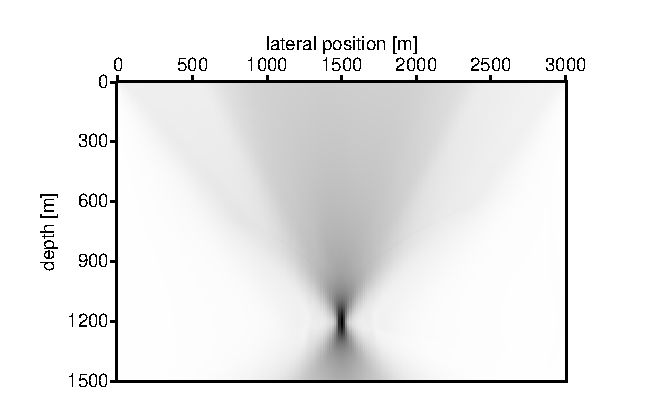
\epsfig{file=EPS/extrap_beam.eps,height=5cm}}
    \put(7.0,-0.3){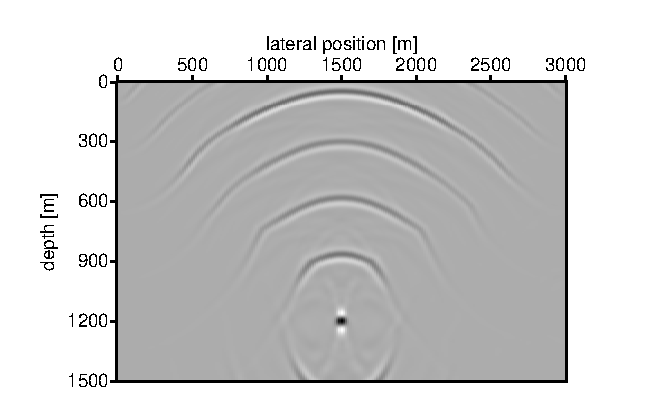
\epsfig{file=EPS/extrap_snap.eps,height=5cm}}
\end{pspicture}
\caption{Inverse extrapolated results of Green's function placed in the middle of the model of Figure \ref{model} at z=1200 m. The
left picture shows the energy beam of the extrapolated wavefield and the right picture show snapshots of the converging wavefield. } \label{extrap1}
\end{figure}
%

For forward extrapolation of the data through the model the following command can be given (to let the extrapolation stop at a certain depth level use the parameter {\tt zrcv=}):

{\footnotesize
\begin{verbatim}
extrap file_in=green.su file_vel=syncline_cp.su verbose=1 mode=-1 zrcv=1200 | suximage 
\end{verbatim}}

Now with cfpmod from surface to depth and then with extrap from depth back to surface:

{\footnotesize
\begin{verbatim}

cfpmod file_vel=syncline_cp.su xsrc1=1500 zsrc1=0 zrcv=1200 ntap=30 file_src=ricker.su file_out=deep.su

extrap file_in=deep.su file_vel=syncline_cp.su verbose=1 zrcv=0 zstart=1200 reverse=1 mode=-1 verbose=1 | suximage 

\end{verbatim}}

%
\begin{figure}[hb]
  \begin{pspicture}(8,5.2)
    \put(-0.5,-0.3){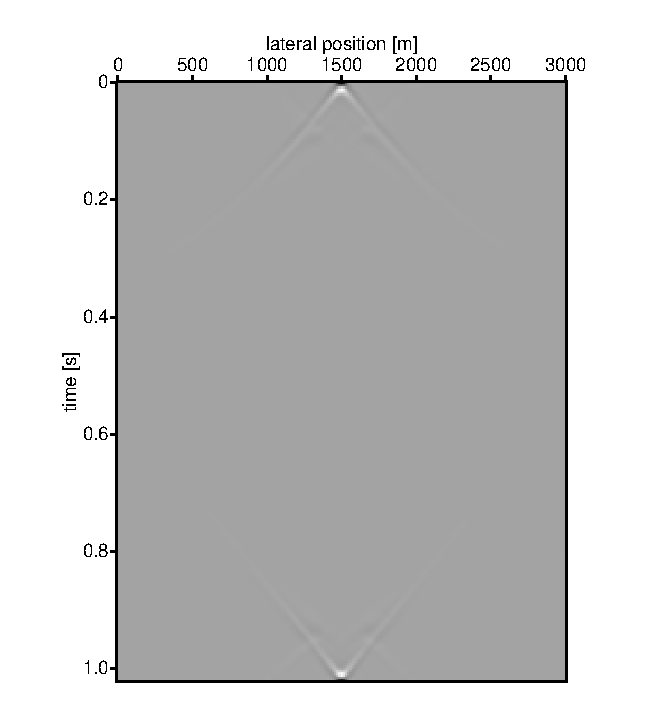
\epsfig{file=EPS/extrap_z1200.eps,height=6cm}}
    \put(7.0,-0.3){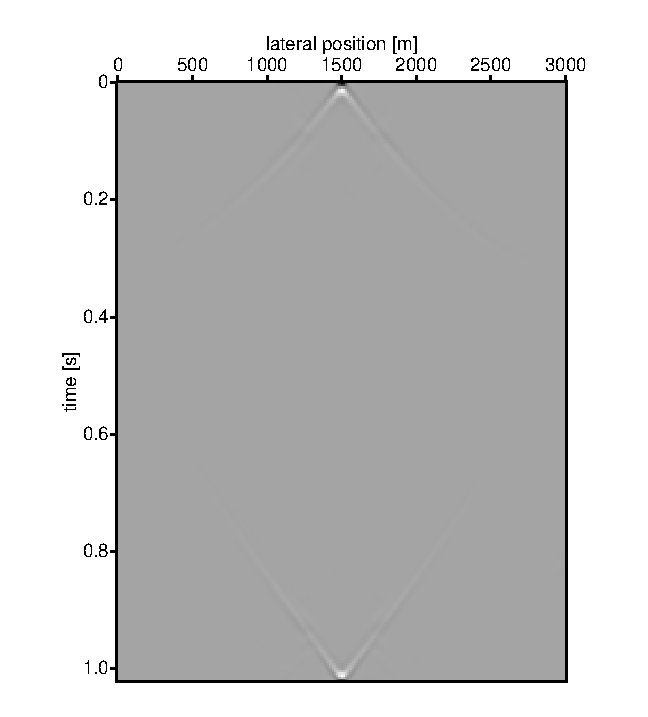
\epsfig{file=EPS/extrap_z0.eps,height=6cm}}
\end{pspicture}
\caption{Inverse extrapolated wavefields of Green's function placed in the middle of the model of Figure \ref{model} at z=1200 m.
(left) the right picture show the result of a source at the surface and receivers at z=1200 m.} \label{extrap2}
\end{figure}
%
\subsection{To do}
Extension of the operator optimization algorithms to 3D media, this extension is already available in a non-official release version and can be obtained on request.

\subsection{References}

Thorbecke, J., Wapenaar, K.,  and Swinnen, G., 2004, Design of one way wavefield extrapolation operators, using smooth functions in WLSQ optimization.: {\bf Geophysics}, pages 1037--1045.

